\documentclass[11pt]{article}
\usepackage[margin=1in]{geometry}
\usepackage{graphicx}
\usepackage{natbib}
\usepackage{hyperref}
\usepackage{booktabs}
\usepackage{dcolumn}
\usepackage{adjustbox}
\usepackage{amsmath}

\begin{document}

\begin{titlepage}
  \begin{center}
    \vspace*{1cm}

    \Huge
    \textbf{Do Banks Price Firms' Data Breaches?}

    \vspace{0.5cm}
    \LARGE
    Huang and Wang (2020)

    \vspace{1.5cm}

    \vfill

    \vspace{0.8cm}

    \Large
    Replication and Report by\
    \textbf{Yunlin FENG}

    \vspace{0.8cm}

    \large
    \today

  \end{center}
\end{titlepage}

\section{Introduction}

This report presents a replication of the paper "Do Banks Price Firms' Data Breaches?" by Huang and Wang, published in The Accounting Review in November 2020. The authors examine how reported data breaches affect firms' bank loan terms. They hypothesize that data breaches lead to higher default risk due to direct costs and reputation loss, as well as higher information risk, resulting in less favorable bank loan terms. The authors use a staggered difference-in-differences approach and find that breached firms experience significantly higher loan spreads, a higher likelihood of collateral requirements, and more covenants compared to control firms.

\section{Replication}

\subsection{Sample Development}
The replication follows the sample development steps outlined in the original paper (with few insignificant omissions). However, due to differences in data availability, the sample size differs slightly from the original study, as shown in Table \ref{tab:sample}. The replication starts with a larger number of data breaches (587) compared to the original study (551) from 2005 (2010) to 2014 (2020). After applying various filters, such as excluding firms with prior breach events, selecting the most significant events, and ensuring data availability for propensity score matching (PSM), the replication study obtains 228 event firms, compared to 213 in the original study. The replication then combines these event firms with matched control firms, resulting in a total of 456 firms, slightly more than the 426 firms in the original study. Finally, after merging with bank loan observations from 2003 (2008) to 2016 (2022) and applying additional filters, the replication study's final sample consists of 1,973 observations involving 149 data breach event firms, compared to 1,081 observations and 139 event firms in the original study.


\begin{table}[ht]
  \centering
  \scriptsize
  \begin{tabular}{@{}lrr@{}}
    \toprule
    \textbf{Step}                                            & \textbf{Authors'} & \textbf{Mine} \\ \midrule
    \# data breaches from 2005 (2010) to 2014 (2020)         & 551               & 587           \\
    Less:                                                    &                   &               \\
    \quad \# firms with a prior breach event                 & (16)              & (9)           \\
    \quad \# events that are not the most significant        & (70)              & (195)         \\
    \quad \# event firms lacking the data for (PSM)          & (252)             & (155)         \\
    \# event firms after PSM                                 & 213               & 228           \\
    event firms + control firms                              & 426               & 456           \\
    Bank loan observations from 2003 (2008) to 2016 (2022)   & 1,428             & 2,165         \\
    Less:                                                    &                   &               \\
    \quad financial services industries                      & (254)             & (166)         \\
    \quad bridge loans and non-fund-based facilities         & (55)              & (NA)          \\
    \quad insufficient to calculate control variables        & (37)              & (26)          \\
    Final sample involving 139 (149) data breach event firms & 1,081             & 1,973         \\ \bottomrule
  \end{tabular}
  \caption{Sample Development}
  \label{tab:sample}
\end{table}

\subsection{Probit Regression}
The first step in the analysis is a probit regression to estimate the propensity scores for matching treatment and control firms. Table \ref{tab:probit} presents the probit regression results, which are largely consistent with the original paper, although some variables are not available in the replication data. Table \ref{tab:diff} presents the differences in variables between the treated and matched control group (replicated values in parenthesis). None of the differences are significant, indicating a succesesful match.

\begin{table}[ht]
  \centering
  \scriptsize
  \begin{tabular}{@{}lcc@{}}
    \toprule
                               & Authors'  & Mine     \\
    \midrule
    Firm Size$_{t-1}$          & 0.154***  & 0.182*** \\
    Leverage$_{t-1}$           & -0.016    & 0.199*   \\
    ROA$_{t-1}$                & 0.089***  & -0.164   \\
    Operational Risk$_{t-1}$   & 0.358*    & 0.761    \\
    Tangibility$_{t-1}$        & -0.005    & -0.331*  \\
    Z-score$_{t-1}$            & -0.086    & 0.002    \\
    MB$_{t-1}$                 & -0.000**  & 0.010    \\
    IT Expertise$_{t-1}$       & 0.233***  & -0.024   \\
    IT Reputation$_{t-1}$      & 0.222**   & NA       \\
    Number of Segments$_{t-1}$ & -0.009    & NA       \\
    ICW$_{t-1}$                & -0.134    & NA       \\
    Intercept                  & -7.881*** & -11.895  \\
    \midrule
    Industry/Year              & Included  & Included \\
    Number of Observations     & 57,462    & 33,157   \\
    Pseudo R$^2$               & 0.166     & 0.243    \\
    \bottomrule
  \end{tabular}
  \caption{Probit Regression Results}
  \label{tab:probit}
\end{table}

\begin{table}[ht]
  \centering
  \scriptsize
  \begin{tabular}{@{}lcccc@{}}
    \toprule
    Variable           & Treated       & Control       & Diff.           & p             \\
    \midrule
    Firm Size          & 8.308 (8.846) & 8.190 (8.752) & 0.118 (0.094)   & 0.591 (0.545) \\
    Leverage           & 0.459 (0.653) & 0.485 (0.679) & -0.026 (-0.026) & 0.768 (0.397) \\
    ROA                & 0.122 (0.134) & 0.124 (0.130) & -0.002 (0.003)  & 0.859 (0.693) \\
    Operational Risk   & 0.059 (0.039) & 0.077 (0.036) & -0.018 (0.002)  & 0.137 (0.472) \\
    Tangibility        & 0.431 (0.237) & 0.449 (0.241) & -0.018 (-0.003) & 0.643 (0.881) \\
    Z-score            & 3.245 (4.965) & 2.129 (4.770) & 1.116 (0.196)   & 0.408 (0.809) \\
    MB                 & 2.330 (1.619) & 2.455 (1.552) & -0.125 (0.067)  & 0.859 (0.683) \\
    IT Expertise       & 0.364 (0.123) & 0.341 (0.105) & 0.023 (0.018)   & 0.616 (0.567) \\
    IT Reputation      & 0.092         & 0.083         & 0.009           & 0.735         \\
    Number of Segments & 2.055         & 1.853         & 0.203           & 0.252         \\
    ICW                & 0.028         & 0.009         & 0.018           & 0.154         \\
    \bottomrule
  \end{tabular}
  \label{tab:diff}
  \caption{Difference in Variables for firms Matched by PSM}
\end{table}

\subsection{Descriptive Statistics}
Table \ref{tab:summary} presents the descriptive statistics of the key variables in the replication sample, which are largely consistent with the original paper (to facilate comparison, only mean is shown). Some differences worth pointing out: \begin{itemize}
  \item The loans in my sample are larger
  \item The loans in my sample are less likely to be secured
  \item The panel is not as balanced in my sample as post-breach loans are fewer than pre-breach loans
\end{itemize}

\begin{table}[ht]
  \centering
  \scriptsize
  \begin{tabular}{@{}lrr@{}}
    Variable                           & \textbf{Authors' Mean} & \textbf{My Mean} \\
    \midrule
    \textit{Bank Loan Characteristics} &                        &                  \\
    \quad Loan Spread                  & 210.500                & 173.673          \\
    \quad Loan Amount                  & 0.954                  & 1.781            \\
    \quad Maturity                     & 55.310                 & 47.196           \\
    \quad Performance Pricing          & 0.423                  & 0.298            \\
    \quad Secured                      & 0.485                  & 0.276            \\
    \quad Total Covenants              & 3.096                  & 5.104            \\

    \textit{Data Breach Variables}     &                        &                  \\
    \quad Breach                       & 0.543                  & 0.568            \\
    \quad Post                         & 0.475                  & 0.375            \\

    \textit{Firm-Level Variables}      &                        &                  \\
    \quad Firm Size                    & 8.779                  & 9.422            \\
    \quad Leverage                     & 0.503                  & 0.650            \\
    \quad          ROA                 & 0.144                  & 0.136            \\
    \quad Operational Risk             & 0.043                  & 0.032            \\
    \quad Tangibility                  & 0.568                  & 0.285            \\
    \quad Z-Score                      & 2.883                  & 3.966            \\
    \quad MB                           & 2.372                  & 1.329            \\
    \quad IT Expertise                 & 0.391                  & 0.114            \\
  \end{tabular}
  \caption{Descriptive Statistics}
  \label{tab:summary}
\end{table}

\subsection{Difference-in-Differences Analysis}
The main analysis uses a staggered difference-in-differences (DiD) approach to examine the effect of data breaches on bank loan terms. The regression specification is as follows:

\begin{align*}
  \text{Loan Contract Terms} & = \beta_0 + \beta_1\text{Data Breach} \times \text{Year}{-1} + \beta_1\text{Data Breach} \times \text{Year}{0} \\
                             & + \beta_1\text{Data Breach} \times \text{Year}{1} + \beta_1\text{Data Breach} \times \text{Year}{2}            \\
                             & + \beta \text{Controls} + \varepsilon
\end{align*}

Table \ref{tab:did} presents the DiD regression results. Unlike the original paper, the replication does not find significant effects of data breaches on bank loan terms.

\begin{table}[ht]
  \centering
  \scriptsize
  \begin{tabular}{@{\extracolsep{5pt}}lD{.}{.}{-3} D{.}{.}{-3} D{.}{.}{-3} }
    \hline
    \hline
                        & \multicolumn{1}{c}{Loan Spread} & \multicolumn{1}{c}{Total Covenants} & \multicolumn{1}{c}{Secured} \\
    \hline
    Breach:Year -1      & 0.009                           & -0.163                              & -0.033                      \\
                        & (0.063)                         & (0.330)                             & (0.041)                     \\
    Breach:Year 0       & -0.010                          & 0.022                               & -0.028                      \\
                        & (0.064)                         & (0.318)                             & (0.041)                     \\
    Breach:Year 1       & -0.031                          & -0.202                              & -0.025                      \\
                        & (0.066)                         & (0.415)                             & (0.045)                     \\
    Breach:Year 2+      & -0.033                          & -0.177                              & 0.008                       \\
                        & (0.045)                         & (0.251)                             & (0.030)                     \\
    Log(Loan Amount)    & -0.018                          & -0.090                              & -0.018^{*}                  \\
                        & (0.016)                         & (0.103)                             & (0.010)                     \\
    Log(Loan Maturity)  & -0.010                          & -0.031                              & 0.066^{***}                 \\
                        & (0.022)                         & (0.124)                             & (0.014)                     \\
    Performance Pricing & 0.082^{***}                     & 0.172                               & 0.043^{**}                  \\
                        & (0.027)                         & (0.136)                             & (0.018)                     \\
    Firm Size           & -0.200^{***}                    & -0.365^{*}                          & -0.037                      \\
                        & (0.037)                         & (0.211)                             & (0.024)                     \\
    Leverage            & 0.844^{***}                     & 1.012                               & 0.203^{**}                  \\
                        & (0.128)                         & (0.922)                             & (0.085)                     \\
    ROA                 & -1.075^{***}                    & -1.156                              & 0.021                       \\
                        & (0.248)                         & (2.257)                             & (0.168)                     \\
    Operational Risk    & 0.309                           & -3.580                              & 0.170                       \\
                        & (0.638)                         & (3.449)                             & (0.418)                     \\
    Tangibility         & 0.309                           & 2.320                               & -0.398^{***}                \\
                        & (0.237)                         & (1.417)                             & (0.154)                     \\
    Z-Score             & 0.029^{*}                       & -0.103                              & -0.012                      \\
                        & (0.016)                         & (0.102)                             & (0.011)                     \\
    MB                  & -0.079^{**}                     & 0.094                               & -0.039^{*}                  \\
                        & (0.031)                         & (0.232)                             & (0.021)                     \\
    IT Expertise        & -0.161^{***}                    & 0.120                               & 0.009                       \\
                        & (0.054)                         & (0.288)                             & (0.034)                     \\
    \hline                                                                                                                    \\[-1.8ex]
    Observations        & \multicolumn{1}{c}{1,608}       & \multicolumn{1}{c}{850}             & \multicolumn{1}{c}{1,889}   \\
  \end{tabular}
  \caption{Difference-in-Differences Regression Results}
  \label{tab:did}
\end{table}

For comparison, Figures \ref{fig:originalDiD} presents the DiD regression results from the original paper.

\begin{figure}[ht]
  \centering
  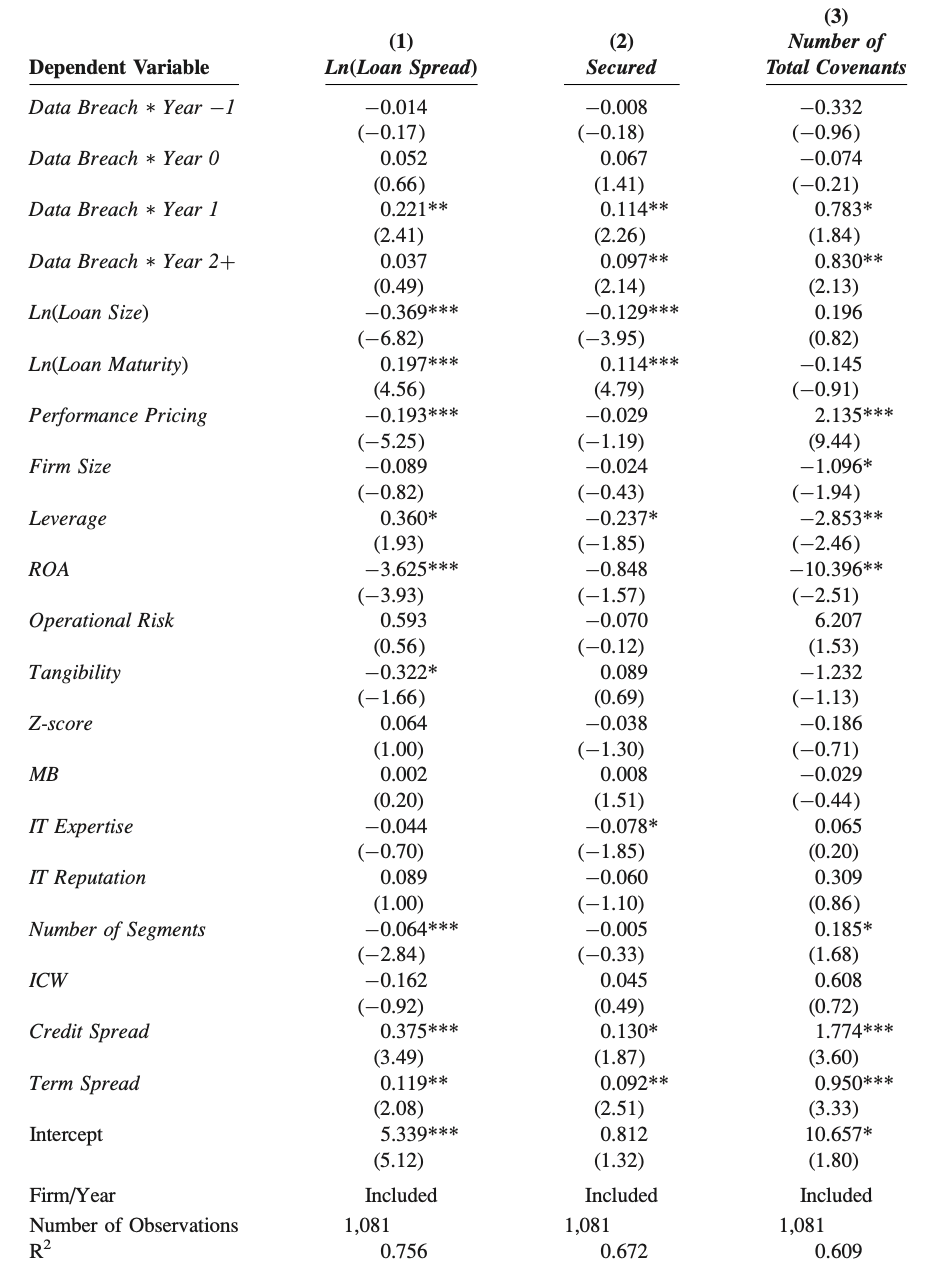
\includegraphics[width=0.8\textwidth]{../tabs/main.png}
  \caption{Original Paper DiD Results}
  \label{fig:originalDiD}
\end{figure}
\section{Conclusion}
The replication study does not find significant effects of data breaches on bank loan terms, in contrast to the original paper. Possible reasons for the discrepancy include: \begin{itemize}
  \item Different data breach databases. The paper's data breach sample is sourced from Privacy Rights Clearinghouse where as mine is based on WRDS. Since my sample are noticeably fewer than the authors', the database may be biased towards certain kinds of data breaches.
  \item Different sample period. My sample is 6 years later than the authors'. Perhaps as data breaches become more prevalent, banks no longer factor it as a risk when writing loans.
  \item Different control variable. Due to time constraint, the replication ignores several control variables such as firm characteristics and macroeconomic data. Including them may yield a different result.
\end{itemize}

\end{document}